%%%%%%%%% INTRODUCTION TO OURL

\begin{frame}{Overview}
	\vspace*{1cm}
	We introduce the action language \emphSlide{\ourL}\\
	\begin{itemize}
		\item[-] Used to describe \mep\ problems
		\item[-] Same syntax of the action language \emphSlide{\mAP}~\cite{baral2015action}
		\item[-] As expressive as \mAP
		\item[-] Uses \posS\ as states
	\end{itemize}
	\begin{tikzpicture}[remember picture,overlay]
		\node[xshift=-4cm,yshift=-7.8cm] at (current page.north east) {
\includegraphics[width=0.4\textwidth]{img/studying_charlie}};
	\end{tikzpicture}
\end{frame}

\begin{frame}{Actions}

	\textbf{Three} types of actions:
	\begin{itemize}
		\onslide<1->{
		{\only<2-3>{\transparent{0.5}}
		\item[-] \only<1>{\emphSlide}{Ontic}: modifies some fluents of the world
		      \begin{itemize}
			      \item[] \only<1>{\ttSlide}{Charlie \emph{opens} the box}
		      \end{itemize}
		      }
		      }
		      \onslide<2->{
		      {\only<3>{\transparent{0.5}}
		\item[-] \only<2>{\emphSlide}{Sensing}: senses the true value of a fluent
		      \begin{itemize}
			      \item[] \only<2>{\ttSlide}{Charlie \emph{peeks} inside the box}
		      \end{itemize}
		      }
		      }
		      \onslide<3->{
		\item[-] \emphSlide{Announcement}:  announces the fluent to other agents
		      \begin{itemize}
			      \item[] \ttSlide{Charlie \emph{announces} the coin position}
		      \end{itemize}
		      }
	\end{itemize}
	\vfill
	\begin{center}
		\only<1>{
\includegraphics[width=0.3\textwidth]{img/open_charlie}}
		\only<2>{
\includegraphics[width=0.3\textwidth]{img/peek_charlie}}
		\only<3>{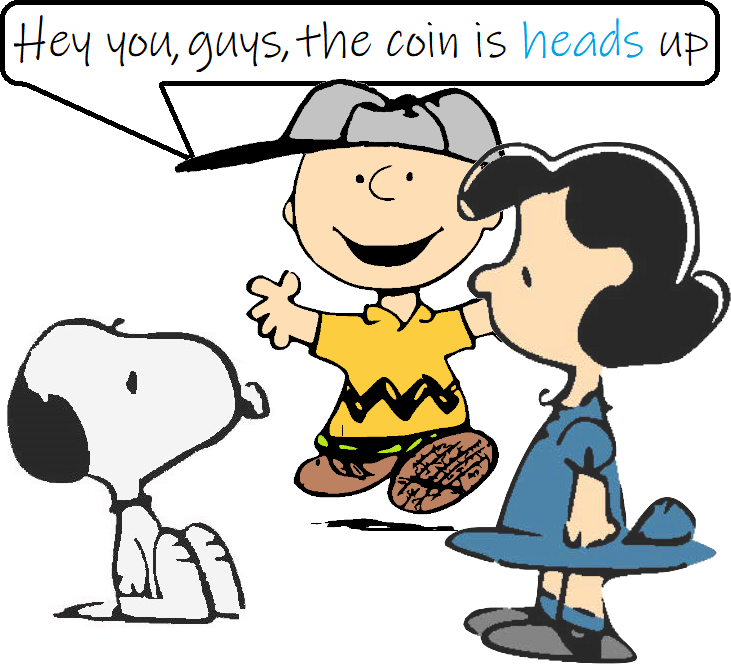
\includegraphics[width=0.4\textwidth]{img/announce_charlie}}
	\end{center}
\end{frame}

\begin{frame}{Observability Relations}
	An \emphSlide{execution} of an action might change or not an agents' belief accordingly to her degree of awareness\\
	\vspace{0.2cm}
	%This because each \textbf{action instance} ($\calA \times \sAG$)  associates an \textbf{observability relation} to each agent:
	\begin{table}
		\centering
		\begin{adjustbox}{width=\columnwidth,center}
			\begin{tabular}{||c||c|c|c||}
				\hhline{|t:=:t:===:t|}
				\multicolumn{1}{||c||}{Action type}
				 & \multicolumn{1}{c|}{\phantom{...}Full observers\phantom{...}}
				 & \multicolumn{1}{c|}{\phantom{..}Partial Observers\phantom{..}}
				 & \multicolumn{1}{c||}{\phantom{...}Oblivious\phantom{...}}      \\
				\hhline{|:=::===:|}
				\multicolumn{1}{||c||}{Ontic}
				 & \multicolumn{1}{c|}{\checkmark}
				 & \multicolumn{1}{c|}{}
				 & \multicolumn{1}{c||}{\checkmark}                               \\
				\hhline{||-||-|-|-||}
				\multicolumn{1}{||c||}{Sensing}
				 & \multicolumn{1}{c|}{\checkmark}
				 & \multicolumn{1}{c|}{\checkmark}
				 & \multicolumn{1}{c||}{\checkmark}                               \\
				\hhline{||-||-|-|-||}
				\multicolumn{1}{||c||}{Announcement}
				 & \multicolumn{1}{c|}{\checkmark}
				 & \multicolumn{1}{c|}{\checkmark}
				 & \multicolumn{1}{c||}{\checkmark}                               \\
				\hhline{|b:=:b:===:b|}
			\end{tabular}
		\end{adjustbox}
	\end{table}
\end{frame}


\begin{frame}{\Pos\ as a state}
	In \ourL\ a state is encoded by a \pos\ where
	\begin{itemize}
		\item[-] (\agentSlide{agent}, $\sigma$) represent the \posS\  believed by \agentSlide{agent}
		\item[-] If \ttSlide{f} $\in \sF$ is present then it is true
	\end{itemize}
	\vspace{1cm}

	\onslide<1->{

		%	{\small Equations are expressed as follows:}\\
		%	\begin{center}
		%		$\poss{u} = \bra{(\agentSlide{ag_1}, \sigma), (\agentSlide{ag_2}, \sigma^\prime), \dots ,\ttSlide{f},$ \ttSlide{f$^\prime$} $, \dots}$\\
		%		{\footnotesize \transparent{0.8} where \agentSlide{ag_1}, \agentSlide{ag_2} $\in \sAG$, $\sigma, \sigma^\prime$ are sets of \posS\ and \ttSlide{f}, \ttSlide{f$^\prime$} $\in \sF$.}}
		%			\end{center}
		\hspace*{-0.2cm}
		$\emphColorSlide{\poss{w}}= \{%
			(\agentSlide{ag},\bra{\poss{w}, \poss{w^\prime}}),%
			(\agentSlide{C},\bra{\poss{v}, \poss{v^\prime}}),%
			\ttSlide{look(\agentSlide{ag})},%
			\ttSlide{key(\agentSlide{A})},%
			\ttSlide{opened},%
			\ttSlide{heads}%
			\}$
		{\footnotesize \transparent{0.8} where \agentSlide{ag} $\in \bra{\agentSlide{A}, \agentSlide{B}}$}
	}
	\begin{center}

	\end{center}
	\vfill
	\onslide<2->{
		\begin{figure}
			\centering
			\hspace*{-0.8cm}
			{%
				\scalebox{.65}%
				{%
					\raisebox{1.5cm}{

						$\begin{aligned}
	&\begin{cases}
		\poss{w}&= \bra{
		  	(\agent{ag},\bra{\poss{w}, \poss{w^\prime}}),
		  	(\agent{c},\bra{\poss{v}, \poss{v^\prime}}),
		  	\looking{ag},
		  	\haskey{a},
		  	\opened%
	  	}\\
		\poss{w^\prime} &=\bra{
		  	(\agent{ag},\bra{\poss{w}, \poss{w^\prime}}),
		  	(\agent{c},\bra{\poss{v}, \poss{v^\prime}}),
		  	\looking{ag},
		  	\haskey{a}, 
		  	\opened, 
		  	\head%
	 	 }\\
		\poss{v} &= \bra{
			(\agent{a},\bra{\poss{v}, \poss{v^\prime}}),
			(\agent{b},\bra{\poss{v}, \poss{v^\prime}}),
			(\agent{c},\bra{\poss{v}, \poss{v^\prime}}),
			\looking{ag},
			\haskey{a}%
		}\\
		\poss{v}^\prime &= \bra{
			(\agent{a},\bra{\poss{v}, \poss{v^\prime}}),
			(\agent{b},\bra{\poss{v}, \poss{v^\prime}}),
			(\agent{c},\bra{\poss{v}, \poss{v^\prime}}),
			\looking{ag},
			\haskey{a},
			\head%
		}\\
	\end{cases}\\
	&\text{where }\agent{ag} \in \bra{\agent{a}, \agent{b}}.
\end{aligned}$



					}%
				}%
			}%
			\scalebox{0.6}{
				\raisebox{0cm}{
					

\tikzset{every picture/.style={line width=0.75pt}} %set default line width to 0.75pt        
\trimbox{0cm 0cm 0cm 1.8cm}{ 

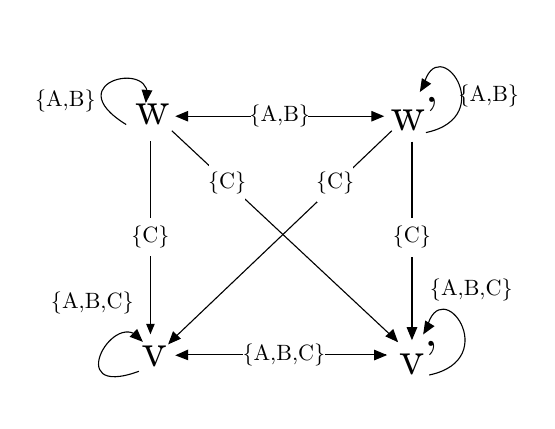
\begin{tikzpicture}[x=0.75pt,y=0.75pt,yscale=-1,xscale=1]
%uncomment if require: \path (0,237.1999969482422); %set diagram left start at 0, and has height of 237.1999969482422

%Straight Lines [id:da49380865843539024] 
\draw    (58,37.52) -- (58,129.88) ;


%Curve Lines [id:da5900505897070274] 
\draw    (55.82,18.4) .. controls (62.62,-2.4) and (11.9,8.32) .. (46.3,29.52) ;


%Shape: Triangle [id:dp7638941010979212] 
\draw  [fill={rgb, 255:red, 0; green, 0; blue, 0 }  ,fill opacity=1 ] (55.82,18.4) -- (54.11,12.94) -- (58.52,13.35) -- cycle ;
%Curve Lines [id:da33896708594278424] 
\draw    (53.81,133.72) .. controls (41.67,115.51) and (14.49,162.32) .. (52.43,148.41) ;


%Shape: Triangle [id:dp06181068467144124] 
\draw  [fill={rgb, 255:red, 0; green, 0; blue, 0 }  ,fill opacity=1 ] (53.81,133.72) -- (48.46,131.68) -- (51.51,128.48) -- cycle ;
%Straight Lines [id:da3518787636435954] 
\draw    (73.3,140.52) -- (171.3,140.52) ;


%Straight Lines [id:da9419961743422685] 
\draw    (167.3,25.52) -- (73.3,25.52) ;


%Straight Lines [id:da5282217469281014] 
\draw    (184,37.72) -- (184,130.08) ;


%Curve Lines [id:da1255493565606156] 
\draw    (191.12,127.8) .. controls (197.84,99.92) and (228.32,142.6) .. (192.32,150.2) ;


%Shape: Triangle [id:dp330887907957337] 
\draw  [fill={rgb, 255:red, 0; green, 0; blue, 0 }  ,fill opacity=1 ] (189.76,130.06) -- (190.59,124.4) -- (194.38,126.68) -- cycle ;
%Curve Lines [id:da19283464821040464] 
\draw    (189.52,11) .. controls (196.24,-16.88) and (226.72,25.8) .. (190.72,33.4) ;


%Shape: Triangle [id:dp48172892570830794] 
\draw  [fill={rgb, 255:red, 0; green, 0; blue, 0 }  ,fill opacity=1 ] (188.16,13.26) -- (188.99,7.6) -- (192.78,9.88) -- cycle ;
%Shape: Triangle [id:dp06884054633092584] 
\draw  [fill={rgb, 255:red, 0; green, 0; blue, 0 }  ,fill opacity=1 ] (184,132.72) -- (181.79,127.43) -- (186.21,127.44) -- cycle ;
%Shape: Triangle [id:dp349860096054311] 
\draw  [fill={rgb, 255:red, 0; green, 0; blue, 0 }  ,fill opacity=1 ] (171.3,140.58) -- (166.02,142.79) -- (166.02,138.37) -- cycle ;
%Shape: Triangle [id:dp5271852980265475] 
\draw  [fill={rgb, 255:red, 0; green, 0; blue, 0 }  ,fill opacity=1 ] (70.66,140.7) -- (75.94,138.31) -- (75.94,142.73) -- cycle ;
%Shape: Triangle [id:dp36308950352931935] 
\draw  [fill={rgb, 255:red, 0; green, 0; blue, 0 }  ,fill opacity=1 ] (58,129.88) -- (56.3,125.81) -- (59.7,125.81) -- cycle ;
%Shape: Triangle [id:dp1292227483684376] 
\draw  [fill={rgb, 255:red, 0; green, 0; blue, 0 }  ,fill opacity=1 ] (70.66,25.52) -- (75.94,23.31) -- (75.94,27.73) -- cycle ;
%Shape: Triangle [id:dp08607057312201727] 
\draw  [fill={rgb, 255:red, 0; green, 0; blue, 0 }  ,fill opacity=1 ] (169.94,25.52) -- (164.66,27.73) -- (164.66,23.31) -- cycle ;
%Straight Lines [id:da22782472852235425] 
\draw    (68.3,32.51) -- (176.84,133.88) ;


%Straight Lines [id:da40972295623496247] 
\draw    (174.3,32.51) -- (68.8,133.01) ;


%Shape: Triangle [id:dp9557525693039122] 
\draw  [fill={rgb, 255:red, 0; green, 0; blue, 0 }  ,fill opacity=1 ] (176.84,133.88) -- (171.64,131.49) -- (174.89,128.49) -- cycle ;
%Shape: Triangle [id:dp9360830131568407] 
\draw  [fill={rgb, 255:red, 0; green, 0; blue, 0 }  ,fill opacity=1 ] (66.99,134.94) -- (69,129.58) -- (72.22,132.61) -- cycle ;

% Text Node
\draw (59,24.32) node [scale=1.7280000000000002] [align=left] {\emphColorSlide{\poss{w}}};
% Text Node
\draw (59.8,141.22) node [scale=1.7280000000000002] [align=left] {\poss{v}};
% Text Node
\draw (17,18.32) node [scale=0.8] [align=left] {\{\agentSlide{A},\agentSlide{B}\}};
% Text Node
\draw (30,115.32) node [scale=0.8] [align=left] {\{\agentSlide{A},\agentSlide{B},\agentSlide{C}\}};
% Text Node
\draw (185.2,24.32) node [scale=1.7280000000000002] [align=left] {\poss{w'}};
% Text Node
\draw (187.11,141.72) node [scale=1.7280000000000002] [align=left] {\poss{v'}};
% Text Node
\draw (212.6,109.32) node [scale=0.8] [align=left] {\{\agentSlide{A},\agentSlide{B},\agentSlide{C}\}};
% Text Node
\draw (221,15.52) node [scale=0.8] [align=left] {\{\agentSlide{A},\agentSlide{B}\}};
% Text Node
\draw  [color={rgb, 255:red, 255; green, 255; blue, 255 }  ,draw opacity=1 ][fill={rgb, 255:red, 255; green, 255; blue, 255 }  ,fill opacity=1 ]  (106.8,16.52) -- (133.8,16.52) -- (133.8,34.52) -- (106.8,34.52) -- cycle  ;
\draw (120.3,25.52) node [scale=0.8,color={rgb, 255:red, 0; green, 0; blue, 0 }  ,opacity=1 ] [align=left] {\{\agentSlide{A},\agentSlide{B}\}};
% Text Node
\draw  [color={rgb, 255:red, 255; green, 255; blue, 255 }  ,draw opacity=1 ][fill={rgb, 255:red, 255; green, 255; blue, 255 }  ,fill opacity=1 ]  (49.5,74.7) -- (66.5,74.7) -- (66.5,92.7) -- (49.5,92.7) -- cycle  ;
\draw (58,83.7) node [scale=0.8,color={rgb, 255:red, 0; green, 0; blue, 0 }  ,opacity=1 ] [align=left] {\{\agentSlide{C}\}};
% Text Node
\draw  [color={rgb, 255:red, 255; green, 255; blue, 255 }  ,draw opacity=1 ][fill={rgb, 255:red, 255; green, 255; blue, 255 }  ,fill opacity=1 ]  (175.5,74.9) -- (192.5,74.9) -- (192.5,92.9) -- (175.5,92.9) -- cycle  ;
\draw (184,83.9) node [scale=0.8,color={rgb, 255:red, 0; green, 0; blue, 0 }  ,opacity=1 ] [align=left] {\{\agentSlide{C}\}};
% Text Node
\draw  [color={rgb, 255:red, 255; green, 255; blue, 255 }  ,draw opacity=1 ][fill={rgb, 255:red, 255; green, 255; blue, 255 }  ,fill opacity=1 ]  (86.5,48.7) -- (103.5,48.7) -- (103.5,66.7) -- (86.5,66.7) -- cycle  ;
\draw (95,57.7) node [scale=0.8,color={rgb, 255:red, 0; green, 0; blue, 0 }  ,opacity=1 ] [align=left] {\{\agentSlide{C}\}};
% Text Node
\draw  [color={rgb, 255:red, 255; green, 255; blue, 255 }  ,draw opacity=1 ][fill={rgb, 255:red, 255; green, 255; blue, 255 }  ,fill opacity=1 ]  (138.5,48.7) -- (155.5,48.7) -- (155.5,66.7) -- (138.5,66.7) -- cycle  ;
\draw (147,57.7) node [scale=0.8,color={rgb, 255:red, 0; green, 0; blue, 0 }  ,opacity=1 ] [align=left] {\{\agentSlide{C}\}};
% Text Node
\draw  [color={rgb, 255:red, 255; green, 255; blue, 255 }  ,draw opacity=1 ][fill={rgb, 255:red, 255; green, 255; blue, 255 }  ,fill opacity=1 ]  (102.8,131.52) -- (141.8,131.52) -- (141.8,149.52) -- (102.8,149.52) -- cycle  ;
\draw (122.3,140.52) node [scale=0.8,color={rgb, 255:red, 0; green, 0; blue, 0 }  ,opacity=1 ] [align=left] {\{\agentSlide{A},\agentSlide{B},\agentSlide{C}\}};


\end{tikzpicture}
}

				}%
			}%
		\end{figure}%
		\begin{center}
			{\footnotesize \transparent{0.8} \Pos\ \emphSlide{\poss{w}} expanded for clarity}
		\end{center}
	}
\end{frame}

\begin{frame}{State equality}
	\begin{itemize}
		\item[-] \PosS\ captures classes of bisimilar Kripke structures
		\item[-] \PosS\ {equality} considers bisimilarity
		\item[-] This help for the \emphSlide{visited states} problem in \mep
	\end{itemize}
	\vfill
	\onslide<2->{
		%\ttSlide{$$\Delta = \peek{B};\distract{B}{C};\flip{C};\tell{B}{C}$$}
		{\footnotesize{\begin{center}
  \poss{r_1}=\bra{
    (\agent{a}, \bra{\poss{s_0}, \poss{s_1}}),
    (\agent{b}, \bra{\poss r_1}),
    (\agent{c}, \bra{\poss r_1}),
    \looking c,
    \haskey{a},
	\opened,
	\head}.
\end{center}
}}
		\begin{figure}
			\centering
			{\scalebox{.37}{\tikzset{every picture/.style={line width=0.75pt}} %set default line width to 0.75pt        

\trimbox{0cm 0cm 0cm 1.8cm}{ 
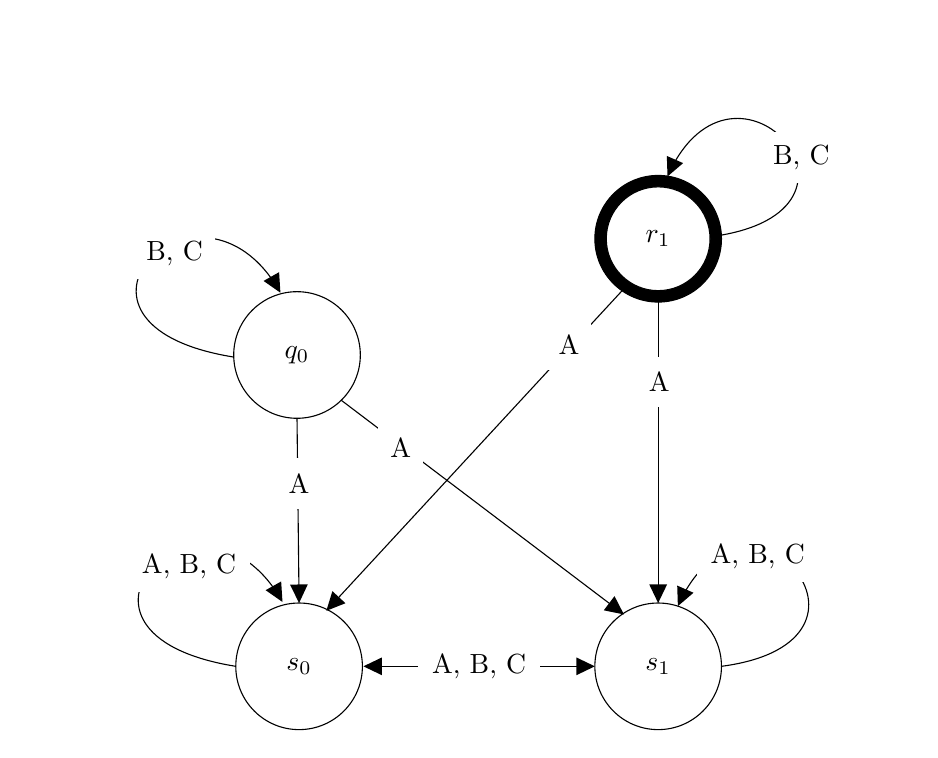
\begin{tikzpicture}[x=0.75pt,y=0.75pt,yscale=-1,xscale=1]
%uncomment if require: \path (0,369); %set diagram left start at 0, and has height of 369

%Shape: Circle [id:dp4758801382807807] 
\draw   (93.5,322) .. controls (93.5,305.16) and (107.16,291.5) .. (124,291.5) .. controls (140.84,291.5) and (154.5,305.16) .. (154.5,322) .. controls (154.5,338.84) and (140.84,352.5) .. (124,352.5) .. controls (107.16,352.5) and (93.5,338.84) .. (93.5,322) -- cycle ;
%Shape: Circle [id:dp5495909764900969] 
\draw   (266.5,322) .. controls (266.5,305.16) and (280.16,291.5) .. (297,291.5) .. controls (313.84,291.5) and (327.5,305.16) .. (327.5,322) .. controls (327.5,338.84) and (313.84,352.5) .. (297,352.5) .. controls (280.16,352.5) and (266.5,338.84) .. (266.5,322) -- cycle ;
%Straight Lines [id:da0065340714279329415] 
\draw    (157,322) -- (264.5,322) ;
\draw [shift={(266.5,322)}, rotate = 180] [fill={rgb, 255:red, 0; green, 0; blue, 0 }  ][line width=0.75]  [draw opacity=0] (8.93,-4.29) -- (0,0) -- (8.93,4.29) -- cycle    ;
\draw [shift={(155,322)}, rotate = 0] [fill={rgb, 255:red, 0; green, 0; blue, 0 }  ][line width=0.75]  [draw opacity=0] (8.93,-4.29) -- (0,0) -- (8.93,4.29) -- cycle    ;
%Curve Lines [id:da8764232980193448] 
\draw    (93.5,322) .. controls (-5.5,306.08) and (76.67,223.33) .. (115.42,289.98) ;
\draw [shift={(116,291)}, rotate = 240.66] [fill={rgb, 255:red, 0; green, 0; blue, 0 }  ][line width=0.75]  [draw opacity=0] (8.93,-4.29) -- (0,0) -- (8.93,4.29) -- cycle    ;

%Curve Lines [id:da9911776319478228] 
\draw    (327.5,322) .. controls (417.91,310.08) and (339.16,221.57) .. (306.98,291.93) ;
\draw [shift={(306.5,293)}, rotate = 293.78] [fill={rgb, 255:red, 0; green, 0; blue, 0 }  ][line width=0.75]  [draw opacity=0] (8.93,-4.29) -- (0,0) -- (8.93,4.29) -- cycle    ;

%Shape: Circle [id:dp7209538961655225] 
\draw  [fill={rgb, 255:red, 0; green, 0; blue, 0 }  ,fill opacity=1 ] (266.5,116) .. controls (266.5,99.16) and (280.16,85.5) .. (297,85.5) .. controls (313.84,85.5) and (327.5,99.16) .. (327.5,116) .. controls (327.5,132.84) and (313.84,146.5) .. (297,146.5) .. controls (280.16,146.5) and (266.5,132.84) .. (266.5,116) -- cycle ;
%Shape: Circle [id:dp27685421107424146] 
\draw   (92.5,172) .. controls (92.5,155.16) and (106.16,141.5) .. (123,141.5) .. controls (139.84,141.5) and (153.5,155.16) .. (153.5,172) .. controls (153.5,188.84) and (139.84,202.5) .. (123,202.5) .. controls (106.16,202.5) and (92.5,188.84) .. (92.5,172) -- cycle ;
%Shape: Circle [id:dp22158231372598314] 
\draw  [fill={rgb, 255:red, 255; green, 255; blue, 255 }  ,fill opacity=1 ] (272,116) .. controls (272,102.19) and (283.19,91) .. (297,91) .. controls (310.81,91) and (322,102.19) .. (322,116) .. controls (322,129.81) and (310.81,141) .. (297,141) .. controls (283.19,141) and (272,129.81) .. (272,116) -- cycle ;
%Straight Lines [id:da40013428570885556] 
\draw    (144.3,193.8) -- (278.91,295.79) ;
\draw [shift={(280.5,297)}, rotate = 217.15] [fill={rgb, 255:red, 0; green, 0; blue, 0 }  ][line width=0.75]  [draw opacity=0] (8.93,-4.29) -- (0,0) -- (8.93,4.29) -- cycle    ;

%Straight Lines [id:da31319417430186725] 
\draw    (281.5,139) -- (138.48,293.78) ;
\draw [shift={(137.13,295.25)}, rotate = 312.74] [fill={rgb, 255:red, 0; green, 0; blue, 0 }  ][line width=0.75]  [draw opacity=0] (8.93,-4.29) -- (0,0) -- (8.93,4.29) -- cycle    ;

%Straight Lines [id:da24005875384214737] 
\draw    (123,202.5) -- (123.98,289.5) ;
\draw [shift={(124,291.5)}, rotate = 269.36] [fill={rgb, 255:red, 0; green, 0; blue, 0 }  ][line width=0.75]  [draw opacity=0] (8.93,-4.29) -- (0,0) -- (8.93,4.29) -- cycle    ;

%Straight Lines [id:da7741558521862318] 
\draw    (297,146.5) -- (297,289.5) ;
\draw [shift={(297,291.5)}, rotate = 270] [fill={rgb, 255:red, 0; green, 0; blue, 0 }  ][line width=0.75]  [draw opacity=0] (8.93,-4.29) -- (0,0) -- (8.93,4.29) -- cycle    ;

%Shape: Circle [id:dp41523883310129905] 
%\draw   (133.5,78) .. controls (133.5,61.16) and (147.16,47.5) .. (164,47.5) .. controls (180.84,47.5) and (194.5,61.16) .. (194.5,78) .. controls (194.5,94.84) and (180.84,108.5) .. (164,108.5) .. controls (147.16,108.5) and (133.5,94.84) .. (133.5,78) -- cycle ;
%Curve Lines [id:da8202719280397651] 
%\draw    (194.5,78) .. controls (284.91,66.08) and (206.16,-22.43) .. (173.98,47.93) ;
%\draw [shift={(173.5,49)}, rotate = 293.78] [fill={rgb, 255:red, 0; green, 0; blue, 0 }  ][line width=0.75]  [draw opacity=0] (8.93,-4.29) -- (0,0) -- (8.93,4.29) -- cycle    ;

%Curve Lines [id:da5631597181878643] 
\draw    (322.5,115) .. controls (412.91,103.08) and (334.16,14.57) .. (301.98,84.93) ;
\draw [shift={(301.5,86)}, rotate = 293.78] [fill={rgb, 255:red, 0; green, 0; blue, 0 }  ][line width=0.75]  [draw opacity=0] (8.93,-4.29) -- (0,0) -- (8.93,4.29) -- cycle    ;

%Curve Lines [id:da7961284231370371] 
\draw    (92.5,173) .. controls (-6.5,157.08) and (75.67,74.33) .. (114.42,140.98) ;
\draw [shift={(115,142)}, rotate = 240.66] [fill={rgb, 255:red, 0; green, 0; blue, 0 }  ][line width=0.75]  [draw opacity=0] (8.93,-4.29) -- (0,0) -- (8.93,4.29) -- cycle    ;

%Straight Lines [id:da052907042750716116] 
%\draw    (177.5,105) -- (279.55,295.24) ;
%\draw [shift={(280.5,297)}, rotate = 241.79] [fill={rgb, 255:red, 0; green, 0; blue, 0 }  ][line width=0.75]  [draw opacity=0] (8.93,-4.29) -- (0,0) -- (8.93,4.29) -- cycle    ;

%Curve Lines [id:da9891597123428996] 
%\draw    (95.16,339.5) .. controls (-58.51,370.39) and (40.01,-87.28) .. (140.5,56) ;

%\draw [shift={(97.5,339)}, rotate = 167.09] [fill={rgb, 255:red, 0; green, 0; blue, 0 }  ][line width=0.75]  [draw opacity=0] (8.93,-4.29) -- (0,0) -- (8.93,4.29) -- cycle    ;

% Text Node
\draw  [color={rgb, 255:red, 255; green, 255; blue, 255 }  ,draw opacity=1 ][fill={rgb, 255:red, 255; green, 255; blue, 255 }  ,fill opacity=1 ]  (181.75,310) -- (239.75,310) -- (239.75,334) -- (181.75,334) -- cycle  ;
\draw (210.75,322) node   {\agent A, \agent B, \agent C};
% Text Node
\draw (124,322) node   {$\defemph  s_{0}$};
% Text Node
\draw (297,322) node   {$\defemph  s_{1}$};
% Text Node
\draw  [color={rgb, 255:red, 255; green, 255; blue, 255 }  ,draw opacity=1 ][fill={rgb, 255:red, 255; green, 255; blue, 255 }  ,fill opacity=1 ]  (42,262) -- (100,262) -- (100,286) -- (42,286) -- cycle  ;
\draw (71,274) node   {\agent A, \agent B, \agent C};
% Text Node
\draw  [color={rgb, 255:red, 255; green, 255; blue, 255 }  ,draw opacity=1 ][fill={rgb, 255:red, 255; green, 255; blue, 255 }  ,fill opacity=1 ]  (316,257) -- (374,257) -- (374,281) -- (316,281) -- cycle  ;
\draw (345,269) node   {\agent A, \agent B, \agent C};
% Text Node
\draw (297,116) node   {$\defemph   r_{1}$};
% Text Node
\draw (123,172) node   {$\defemph  q_{0}$};
% Text Node
%\draw (164,78) node   {$\defemph  r_{1}$};
% Text Node
%\draw  [color={rgb, 255:red, 255; green, 255; blue, 255 }  ,draw opacity=1 ][fill={rgb, 255:red, 255; green, 255; blue, 255 }  ,fill opacity=1 ]  (213,27) -- (251,27) -- (251,51) -- (213,51) -- cycle  ;
%\draw (232,39) node   {\agent B, \agent C};
% Text Node
\draw  [color={rgb, 255:red, 255; green, 255; blue, 255 }  ,draw opacity=1 ][fill={rgb, 255:red, 255; green, 255; blue, 255 }  ,fill opacity=1 ]  (243.5,155) -- (264.5,155) -- (264.5,179) -- (243.5,179) -- cycle  ;
\draw (254,167) node   {\agent A};
% Text Node
\draw  [color={rgb, 255:red, 255; green, 255; blue, 255 }  ,draw opacity=1 ][fill={rgb, 255:red, 255; green, 255; blue, 255 }  ,fill opacity=1 ]  (287,173) -- (308,173) -- (308,197) -- (287,197) -- cycle  ;
\draw (297.5,185) node   {\agent A};
% Text Node
%\draw  [color={rgb, 255:red, 255; green, 255; blue, 255 }  ,draw opacity=1 ][fill={rgb, 255:red, 255; green, 255; blue, 255 }  ,fill opacity=1 ]  (194.5,139) -- (215.5,139) -- (215.5,163) -- (194.5,163) -- cycle  ;
%\draw (205,151) node   {\agent A};
% Text Node
\draw  [color={rgb, 255:red, 255; green, 255; blue, 255 }  ,draw opacity=1 ][fill={rgb, 255:red, 255; green, 255; blue, 255 }  ,fill opacity=1 ]  (113.5,222) -- (134.5,222) -- (134.5,246) -- (113.5,246) -- cycle  ;
\draw (124,234) node   {\agent A};
% Text Node
\draw  [color={rgb, 255:red, 255; green, 255; blue, 255 }  ,draw opacity=1 ][fill={rgb, 255:red, 255; green, 255; blue, 255 }  ,fill opacity=1 ]  (162.5,205) -- (183.5,205) -- (183.5,229) -- (162.5,229) -- cycle  ;
\draw (173,217) node   {\agent A};
% Text Node
\draw  [color={rgb, 255:red, 255; green, 255; blue, 255 }  ,draw opacity=1 ][fill={rgb, 255:red, 255; green, 255; blue, 255 }  ,fill opacity=1 ]  (347,65) -- (385,65) -- (385,89) -- (347,89) -- cycle  ;
\draw (366,77) node   {\agent B, \agent C};
% Text Node
\draw  [color={rgb, 255:red, 255; green, 255; blue, 255 }  ,draw opacity=1 ][fill={rgb, 255:red, 255; green, 255; blue, 255 }  ,fill opacity=1 ]  (45,111) -- (83,111) -- (83,135) -- (45,135) -- cycle  ;
\draw (64,123) node   {\agent B, \agent C};
% Text Node
%\draw  [color={rgb, 255:red, 255; green, 255; blue, 255 }  ,draw opacity=1 ][fill={rgb, 255:red, 255; green, 255; blue, 255 }  ,fill opacity=1 ]  (46.5,48) -- (67.5,48) -- (67.5,72) -- (46.5,72) -- cycle  ;
%\draw (57,60) node   {\agent A};


\end{tikzpicture}
}}}
			\hfill
			{\scalebox{0.37}{\tikzset{every picture/.style={line width=0.75pt}} %set default line width to 0.75pt        
\trimbox{0cm 0cm 0cm 1.8cm}{ 
\begin{tikzpicture}[x=0.75pt,y=0.75pt,yscale=-1,xscale=1]
%uncomment if require: \path (0,332); %set diagram left start at 0, and has height of 332

%Shape: Circle [id:dp09506861109760789] 
\draw   (67.5,279.5) .. controls (67.5,262.66) and (81.16,249) .. (98,249) .. controls (114.84,249) and (128.5,262.66) .. (128.5,279.5) .. controls (128.5,296.34) and (114.84,310) .. (98,310) .. controls (81.16,310) and (67.5,296.34) .. (67.5,279.5) -- cycle ;
%Shape: Circle [id:dp3674876277032001] 
\draw   (240.5,279.5) .. controls (240.5,262.66) and (254.16,249) .. (271,249) .. controls (287.84,249) and (301.5,262.66) .. (301.5,279.5) .. controls (301.5,296.34) and (287.84,310) .. (271,310) .. controls (254.16,310) and (240.5,296.34) .. (240.5,279.5) -- cycle ;
%Straight Lines [id:da686791560478396] 
\draw    (131,279.5) -- (238.5,279.5) ;
\draw [shift={(240.5,279.5)}, rotate = 180] [fill={rgb, 255:red, 0; green, 0; blue, 0 }  ][line width=0.75]  [draw opacity=0] (8.93,-4.29) -- (0,0) -- (8.93,4.29) -- cycle    ;
\draw [shift={(129,279.5)}, rotate = 0] [fill={rgb, 255:red, 0; green, 0; blue, 0 }  ][line width=0.75]  [draw opacity=0] (8.93,-4.29) -- (0,0) -- (8.93,4.29) -- cycle    ;
%Curve Lines [id:da3133467592132765] 
\draw    (67.5,279.5) .. controls (-31.5,263.58) and (50.67,180.83) .. (89.42,247.48) ;
\draw [shift={(90,248.5)}, rotate = 240.66] [fill={rgb, 255:red, 0; green, 0; blue, 0 }  ][line width=0.75]  [draw opacity=0] (8.93,-4.29) -- (0,0) -- (8.93,4.29) -- cycle    ;

%Curve Lines [id:da09866336174690571] 
\draw    (301.5,279.5) .. controls (391.91,267.58) and (313.16,179.07) .. (280.98,249.43) ;
\draw [shift={(280.5,250.5)}, rotate = 293.78] [fill={rgb, 255:red, 0; green, 0; blue, 0 }  ][line width=0.75]  [draw opacity=0] (8.93,-4.29) -- (0,0) -- (8.93,4.29) -- cycle    ;

%Shape: Circle [id:dp9019764791073822] 
\draw  [fill={rgb, 255:red, 0; green, 0; blue, 0 }  ,fill opacity=1 ] (240.5,73.5) .. controls (240.5,56.66) and (254.16,43) .. (271,43) .. controls (287.84,43) and (301.5,56.66) .. (301.5,73.5) .. controls (301.5,90.34) and (287.84,104) .. (271,104) .. controls (254.16,104) and (240.5,90.34) .. (240.5,73.5) -- cycle ;
%Shape: Circle [id:dp23164546006052256] 
\draw  [fill={rgb, 255:red, 255; green, 255; blue, 255 }  ,fill opacity=1 ] (246,73.5) .. controls (246,59.69) and (257.19,48.5) .. (271,48.5) .. controls (284.81,48.5) and (296,59.69) .. (296,73.5) .. controls (296,87.31) and (284.81,98.5) .. (271,98.5) .. controls (257.19,98.5) and (246,87.31) .. (246,73.5) -- cycle ;
%Straight Lines [id:da3406951202857561] 
\draw    (255.5,96.5) -- (112.48,251.28) ;
\draw [shift={(111.13,252.75)}, rotate = 312.74] [fill={rgb, 255:red, 0; green, 0; blue, 0 }  ][line width=0.75]  [draw opacity=0] (8.93,-4.29) -- (0,0) -- (8.93,4.29) -- cycle    ;

%Straight Lines [id:da5969218919849798] 
\draw    (271,104) -- (271,247) ;
\draw [shift={(271,249)}, rotate = 270] [fill={rgb, 255:red, 0; green, 0; blue, 0 }  ][line width=0.75]  [draw opacity=0] (8.93,-4.29) -- (0,0) -- (8.93,4.29) -- cycle    ;

%Curve Lines [id:da32162073734028385] 
\draw    (296.5,72.5) .. controls (386.91,60.58) and (308.16,-27.93) .. (275.98,42.43) ;
\draw [shift={(275.5,43.5)}, rotate = 293.78] [fill={rgb, 255:red, 0; green, 0; blue, 0 }  ][line width=0.75]  [draw opacity=0] (8.93,-4.29) -- (0,0) -- (8.93,4.29) -- cycle    ;


% Text Node
\draw  [color={rgb, 255:red, 255; green, 255; blue, 255 }  ,draw opacity=1 ][fill={rgb, 255:red, 255; green, 255; blue, 255 }  ,fill opacity=1 ]  (155.75,267.5) -- (213.75,267.5) -- (213.75,291.5) -- (155.75,291.5) -- cycle  ;
\draw (184.75,279.5) node   {\agent{A},\agent{B},\agent{C}};
% Text Node
\draw (98,279.5) node   {\defemph{s_{0}}};
% Text Node
\draw (271,279.5) node   {\defemph{s_{1}}};
% Text Node
\draw  [color={rgb, 255:red, 255; green, 255; blue, 255 }  ,draw opacity=1 ][fill={rgb, 255:red, 255; green, 255; blue, 255 }  ,fill opacity=1 ]  (16,219.5) -- (74,219.5) -- (74,243.5) -- (16,243.5) -- cycle  ;
\draw (45,231.5) node   {\agent{A},\agent{B},\agent{C}};
% Text Node
\draw  [color={rgb, 255:red, 255; green, 255; blue, 255 }  ,draw opacity=1 ][fill={rgb, 255:red, 255; green, 255; blue, 255 }  ,fill opacity=1 ]  (290,214.5) -- (348,214.5) -- (348,238.5) -- (290,238.5) -- cycle  ;
\draw (319,226.5) node   {\agent{A},\agent{B},\agent{C}};
% Text Node
\draw (271,73.5) node   {\defemph{r_{1}}};
% Text Node
\draw  [color={rgb, 255:red, 255; green, 255; blue, 255 }  ,draw opacity=1 ][fill={rgb, 255:red, 255; green, 255; blue, 255 }  ,fill opacity=1 ]  (217.5,112.5) -- (238.5,112.5) -- (238.5,136.5) -- (217.5,136.5) -- cycle  ;
\draw (228,124.5) node   {\agent{A}};
% Text Node
\draw  [color={rgb, 255:red, 255; green, 255; blue, 255 }  ,draw opacity=1 ][fill={rgb, 255:red, 255; green, 255; blue, 255 }  ,fill opacity=1 ]  (261,130.5) -- (282,130.5) -- (282,154.5) -- (261,154.5) -- cycle  ;
\draw (271.5,142.5) node   {\agent{A}};
% Text Node
\draw  [color={rgb, 255:red, 255; green, 255; blue, 255 }  ,draw opacity=1 ][fill={rgb, 255:red, 255; green, 255; blue, 255 }  ,fill opacity=1 ]  (321,22.5) -- (359,22.5) -- (359,46.5) -- (321,46.5) -- cycle  ;
\draw (340,34.5) node   {\agent{B},\agent{C}};


\end{tikzpicture}}}}
		\end{figure}
	}
\end{frame}

\subsection*{Entailment}
\begin{frame}{Entailment}
	Let $\varphi,\varphi_{1},\varphi_{2}$ be beliefs formula and \poss{u} be a \pos
	\begin{block}{Entailment w.r.t. \posS}
			\begin{itemize}[<+->]
			\item[-] $\poss{u} \models \ttSlide{l}$ if $\possarg{u}{\ttSlide{l}}= 1$;
			%\item $\poss{u} \models \neg \phi$ if $\poss{u} \not \models \phi$;
			%\item $\poss{u} \models \phi_1 \vee \phi_2$ if $\poss{u} \models
			%	      \phi_1$ or $\poss{u} \models \phi_2$;
			%\item $\poss{u} \models \phi_1 \wedge \phi_2$ if $\poss{u} \models
			%	      \phi_1$ and $\poss{u} \models \phi_2$.
			\item[-] $\poss{u} \models \bBSlide{\agentSlide{ag}}{\varphi}$ if for each $\poss{v} \in \possarg{u}{\agentSlide{ag}}$, $\poss{v} \models \varphi$;
			      %\item $\poss{u} \models \neg \varphi$ if $\poss{u} \not\models \varphi$;
		%	\item $\poss{u} \models \varphi_1 \vee \varphi_2$ if $\poss{u} \models \varphi_1$ or $\poss{u}\models \varphi_2$;
		%	\item $\poss{u} \models \varphi_1 \wedge \varphi_2$ if $\poss{u} \models \varphi_1$ and $\poss{u}\models \varphi_2$;
			\item[-] $\poss{u} \models \eAlpha{\varphi}$ if $\poss{u} \models
				      \bB{ag}{\varphi}$ for all $\agentSlide{ag} \in \alpha$;
			\item<.->[-] $\poss{u} \models \cAlpha{\varphi}$ if
			      $\poss{u} \models \eAlphaIter{k}{\varphi}$ for every
			      $k\geq0$, where $\eAlphaIter{0}{\varphi} = \varphi$ and
			      $\eAlphaIter{k+1}{\varphi}=\eAlpha{(\eAlphaIter{k}{\varphi})}$.
		\end{itemize}
	\end{block}
		\onslide<3->{The entailment for the standard operators is defined as usual}
\end{frame}

\subsection*{Transition function}
\begin{frame}{Ontic Actions}
	
	\begin{block}{$\trfunc$ for Ontic Actions \hfill $\trfunc: \ai\times\Sigma \rightarrow \Sigma \cup \bra{\emptyset}$}
	
	Let \texttt{a} be an \emphSlide{ontic action} instance, \poss{u} a \pos\ and \ttSlide{l} be \ttSlide{f} or \ttSlide{$\neg$}\ttSlide{f}\\
			\vspace{0.2cm}
	\begin{tabular}{rl}
		$\trfunc(\texttt{a}, \poss{u}) =  \emptyset$ &if \texttt{a} is not executable in \poss{u}\\
		$\trfunc( \texttt{a}, \poss{u}) = \poss{v}$& if \texttt{a} \emphSlide{modifies} the \ttSlide{literals} $\in$ \res{a}\\
	\end{tabular}
	
	\vspace{0.65cm}
	Where \poss{v} is\\
		\vspace{0.2cm}
		      $\begin{cases}
				      \possarg{v}{\ttSlide{l}} = \possarg{u}{\ttSlide{l}} & \text{ if } \ttSlide{l} \not\in \res{a} \\
				      \possarg{v}{\ttSlide{l}} = \resSlide{a}{l}                  & \text{ if } \ttSlide{l} \in \res{a}  
				      %\res a &\text{ if } \defemph{f} \in \res{a}
			      \end{cases}$
		      \vspace*{0.2cm}
		      \\and
		      \vspace*{0.2cm}
		      \\
		      $\begin{cases}
				      \possarg{v}{\agentSlide{ag}} = \possarg{u}{\agentSlide{ag}}                                                        & \text{ if } \agentSlide{ag} \in \posoblivious \\
				      \possarg{v}{\agentSlide{ag}} = \bigcup_{\poss{w} \in \possarg{u}{\agentSlide{ag}}} \trfunc( \texttt{a}, \poss{w}) & \text{ if } \agentSlide{ag} \in \posfull
			      \end{cases}$
			    \end{block}

\end{frame}


\begin{frame}{Sensing Actions}
	
	\begin{block}{$\trfunc$ for Sensing Actions \hfill $\trfunc: \ai\times\Sigma \rightarrow \Sigma \cup \bra{\emptyset}$}
		
		Let \texttt{a} be an \emphSlide{sensing action} instance, and \poss{u} a \pos\  and \ttSlide{l} be \ttSlide{f} or \ttSlide{$\neg$}\ttSlide{f}\\
		\vspace{0.2cm}
		\begin{tabular}{rl}
			$\trfunc(\texttt{a}, \poss{u}) =  \emptyset$ &if \texttt{a} is not executable in \poss{u}\\
			$\trfunc( \texttt{a}, \poss{u}) = \poss{v}$& if the literal \ttSlide{l} is \emphSlide{sensed}\\
		\end{tabular}
		
		\vspace{0.65cm}
		Where \poss{v} is\\
		\vspace{0.2cm}
		$\begin{cases}
		\emptyset & \text{if } \sensedSlide{a}{l} \neq \possarg{u}{\ttSlide{l}}\\
		\possarg{v}{\agentSlide{ag}} = \possarg{u}{\agentSlide{ag}}                                                                                                   & \text{if } \agentSlide{ag} \in \posoblivious\\
		\possarg{v}{\agentSlide{ag}} = \bigcup_{\poss{w} \in \possarg{u}{\agentSlide{ag}}} \trfunc( \defemph{a}, \poss{w}) & \text{if }\agentSlide{ag} \in \posfull\\
		\possarg{v}{\agentSlide{ag}} = \bigcup_{\poss{w} \in \possarg{u}{\agentSlide{ag}}} (\trfunc( \defemph{a}, \poss{w}) \cup \trfunc( \neg\defemph{a}, \poss{w})) & \text{if }\agentSlide{ag} \in \pospartial
		\end{cases}$
	\end{block}
	
\end{frame}


\begin{frame}{Announcement Actions}
	
	\begin{block}{$\trfunc$ for Announcement Actions \hfill $\trfunc: \ai\times\Sigma \rightarrow \Sigma \cup \bra{\emptyset}$}
		
		Let \texttt{a} be an \emphSlide{announcement action} instance, and \poss{u} a \pos.\\
		\vspace{0.2cm}
		\begin{tabular}{rl}
			$\trfunc(\texttt{a}, \poss{u}) =  \emptyset$ &if \texttt{a} is not executable in \poss{u}\\
			$\trfunc( \texttt{a}, \poss{u}) = \poss{v}$& if the fluent formula \ttSlide{$\phi$} is \emphSlide{announced}\\
		\end{tabular}
		
		\vspace{0.65cm}
		Where \poss{v} is\\
		\vspace{0.2cm}
		$\begin{cases}
	\emptyset & \text{if } \poss{u} \not \models \phi\\
		\possarg{v}{\agentSlide{ag}} = \possarg{u}{\agentSlide{ag}}                                                                                                   & \text{if } \agentSlide{ag} \in \posoblivious\\
		\possarg{v}{\agentSlide{ag}} = \bigcup_{\poss{w} \in \possarg{u}{\agentSlide{ag}}} \trfunc( \defemph{a}, \poss{w}) & \text{if }\agentSlide{ag} \in \posfull\\
		\possarg{v}{\agentSlide{ag}} = \bigcup_{\poss{w} \in \possarg{u}{\agentSlide{ag}}} (\trfunc( \defemph{a}, \poss{w}) \cup \trfunc( \neg\defemph{a}, \poss{w})) & \text{if }\agentSlide{ag} \in \pospartial
		\end{cases}$
	\end{block}
	
\end{frame}